\chapter{Thickness One}

While results from the previous chapters resolve the question of $m(a_1,a_2,a_3,3)$ for $a_1 \geq a_2 \geq a_3 \geq 11$, similar constructions for smaller grids remain sparse. Nevertheless, computer examples seem to suggest that grids of minimum size at least 2 are largely optimal. Grids of thickness 1 tell a different story. In this chapter, we prove that the only perfect grids in thickness 1 are those of the form $[2^n-1]^2$. This answers a question posed by Benevides et al. in \cite{benevides}.

\section{A tight result for $[n]^2$}
The argumentative structure of the proof is as follows: Let $A_0$ be a perfect lethal set on the grid $(a_1, a_2, 1)$. We show that the structure of $A_0$ guarantees the existence of a perfect lethal set on the smaller grid $(\frac{a_1-1}{2}, \frac{a_2-1}{2}, 1)$. Repeated applications of this process of reduction guarantee the existence of a perfect lethal set on the grid $(a_0, 1,1)$. Since the only such grid that admits a perfect lethal set is $(1,1,1)$, we are forced to conclude that $a_1 = a_2 = 2^k-1$ for some $k > 0$. 

\subsection{Preliminaries}
For the remainder of the chapter, let $G = [a_1] \times [a_2]$. Recall that perfect lethal sets match the surface area bound. In particular,
$$|A_0| = \frac{a_1a_2 + a_1 + a_2}{3}.$$
We begin with the following observations regarding the structure of $A_0$:

\begin{prop}
\label{prop:alternating_border}
If $A_0$ is a perfect lethal set on $G$, then $A_0$ contains alternating vertices along the border of $G$. 
\end{prop}

\begin{proof}
Since $A_0$ is perfect, it must form an independent set in $G$. By Proposition \ref{prop:border}, no two adjacent border vertices are both uninfected. Together, these conditions ensure that $A_0$ intersects the border of $G$ in an alternating pattern (see Figure \ref{fig:border}). 
\end{proof}

\begin{figure}[]
\centering
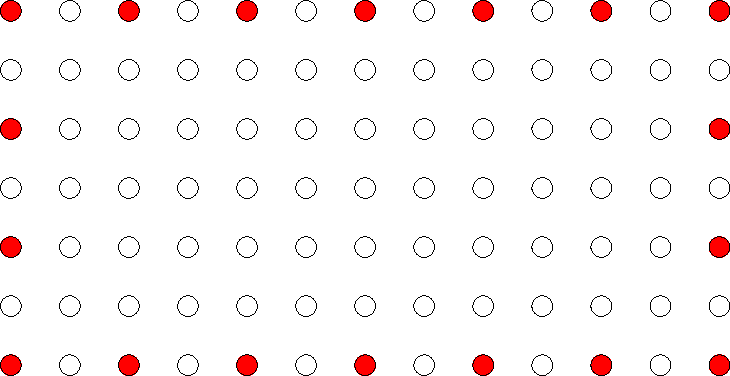
\includegraphics[width=0.5\textwidth]{figures/6/border.pdf}
\caption{Alternating infection along the border of $[7] \times [13]$.}
\label{fig:border}
\end{figure} 

\begin{prop}
\label{prop:odd_by_odd}
If $A_0$ is a perfect lethal set on $G$, then $a_1, a_2 \equiv 1 \pmod 2$.
\end{prop}

\begin{proof}
By Propositions \ref{prop:alternating_border} and \ref{prop:corners}, $a_1, a_2 \equiv 1 \pmod 2$.
\end{proof}

\begin{prop}
\label{prop:one_border_vertex}
Let $A_0$ be a perfect lethal set on $[a_1] \times [a_2]$ under 3-neighbor percolation. Let $H = V([a_1] \times [a_2]) \setminus A_0$. Then the subgraph induced by $H$ is acyclic and each component of $H$ contains exactly one border vertex.
\end{prop}

\begin{proof}
Sufficiency follows from Proposition \ref{prop:immune_regions}. For necessity, observe that the interior vertices of $A_0$ each remove exactly 4 edges from the subgraph induced by $H$. This implies that the subgraph induced by $H$ is a forest with exactly $a_1 + a_2 - 2$ components. As there are exactly $a_1 + a_2 - 2$ border vertices in $H$, each component must contain exactly one border vertex.
\end{proof}

Consider a labeling of the vertices of $G$ by their coordinates, starting at $(1,1)$ in the lower left and ranging to $(a_1,a_2)$ in the upper right. Refer to a vertex $(x,y)$ as ``even" or ``odd" depending on the parity of $x+y$. If a set $S \subseteq V(G)$ contains all vertices of the same parity, call $S$ monochromatic. The following lemma leverages the prior propositions to prove that any perfect lethal set on $G$ must be monochromatic.

\begin{lem}
Let $A_0$ be a perfect lethal set on $G$. Then $A_0$ is monochromatic with respect to the proper 2-coloring of $G$.
\end{lem}

\begin{proof}
From Proposition \ref{prop:alternating_border}, observe that $A_0$ contains all even vertices along the border of $G$. Suppose for contradiction that $A_0$ also contains odd vertices. We show that this implies the existence of a cycle in the subgraph induced by $V(G) \setminus A_0$, contradicting Proposition \ref{prop:one_border_vertex}. 

Let $H$ be a graph with vertices $V(H) = V(G)$ and edges $uv$ if and only if $u$ and $v$ are diagonally adjacent in $G$. Consider the subgraph of $H$ induced by the odd vertices of $A_0$ and let $K$ be a connected component. Observe that $K$ is acyclic: any cycle in $K$ encloses a component of $G[\overline{A_0}]$, contradicting Proposition \ref{prop:one_border_vertex}. Furthermore, by Proposition \ref{prop:alternating_border}, all vertices of $K$ are in the interior of $G$. Let $C_H$ be the cycle induced in $H$ by $N_G(K)$. Note that since $A_0$ is an independent set, $N_G(K) \cap A_0 = \emptyset$ and $C_H \cap A_0 = \emptyset$. Consider the closed walk induced in $G$ by the vertices $V(C_H) \cup N_H(K) \setminus A_0$. This walk describes a cycle $C_G$ in $G[\overline{A_0}]$, which contradicts Proposition \ref{prop:one_border_vertex}.
 \end{proof}

\begin{figure}[]
\centering
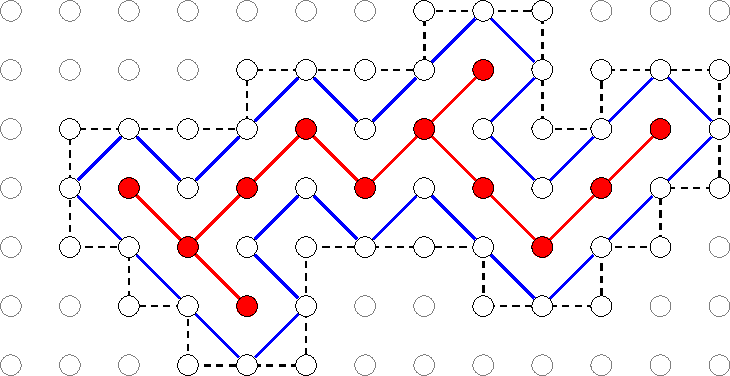
\includegraphics[width=0.5\textwidth]{figures/6/monochromatic.pdf}
\caption{$[7] \times [13]$ grid with component $K$ (red), $C_H$ (blue), and $C_G$ (dashed).}
\label{fig:border}
\end{figure} 

\subsection{Reduction}
We present an auxiliary $(\frac{a_1-1}{2}, \frac{a_2-1}{2}, 1)$ grid $G'$ obtained from $G$, and show that it admits a perfect lethal set. Let the vertices of $G'$ be $2 \times 2$ tiles of $G$ given by
$$\{(2x-1,2y-1),(2x-1,2y),(2x,2y-1),(2x,2y) \mid (x,y) \in [1, (a_1-1)/2] \times [1, (a_2-1)/2]\},$$
with adjacencies between tiles that differ by one in each of the cardinal directions. Note that Proposition \ref{prop:odd_by_odd} ensures that $|V(G')|$ is an integer. Furthermore, observe that for any tile $T_{x,y} \in V(G')$, $|A_0 \cap T_{x,y}| \in \{1,2\}$. This follows from the fact that $A_0$ is an independent set, and $G[\overline{A_0}]$ is acyclic. For all $T_{x,y} \in V(G')$, color $T_{x,y}$ blue if $|A_0 \cap T_{x,y}| = 2$, and white otherwise. Let $b$ and $w$ be the number of blue and white tiles in $V(G')$, respectively. We determine $b$ by solving the following system of equations:
\begin{align*}
b + w &= \frac{(a_1-1)(a_2-1)}{4} \\
2b + w &= \frac{a_1a_2+a_1+a_2}{3} - \frac{a_1+a_2}{2}.
\end{align*}
This gives the following expression for $b$:
\begin{align}
\frac{a_1a_2+a_1+a_2}{3} - \frac{a_1+a_2}{2} - \frac{(a_1-1)(a_2-1)}{4} &= \frac{a_1a_2+a_1+a_2-3}{12} \label{eq:tile_bound_1} \\
&= \frac{(\frac{a_1-1}{2})(\frac{a_2-1}{2}) + \frac{a_1-1}{2} + \frac{a_2-1}{2}}{3} \label{eq:tile_bound_2}.
\end{align}
Note that this is precisely the surface area bound for the $(\frac{a_1-1}{2}, \frac{a_2-1}{2}, 1)$ grid. Furthermore, since $a_1 \equiv a_2 \equiv 1 \pmod 6$ or $a_1 \equiv a_2 \equiv 3 \pmod 6$, all terms on the LHS of \ref{eq:tile_bound_1} are integral, and so the SA bound in \ref{eq:tile_bound_2} is tight.

\begin{figure}[]
\centering
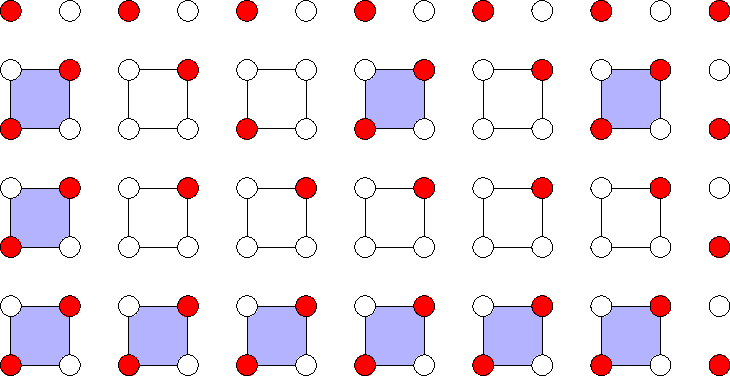
\includegraphics[width=0.5\textwidth]{figures/6/tiles.pdf}
\caption{$[7] \times [13]$ grid with $T_{x,y}$ colored blue if $|T_{x,y} \cap A_0| = 2$. Note that $A_0$ is \emph{not} perfect.}
\label{fig:tiles}
\end{figure} 

We prove that the blue tiles form a lethal set in $G'$. We begin with the following observation:

\begin{prop}
All white tiles have their $A_0$-vertex in the bottom left corner.
\end{prop}

\begin{proof}
For contradiction, suppose that there exists a white tile $T_0$ with one infected vertex in the upper right. By Proposition \ref{prop:one_border_vertex}, there exists a path in $G[\overline{A_0}]$ from $T_0 \setminus A_0$ to the border. We consider the sequence of white tiles $T_0...T_n$ containing this path. 

Consider two consecutive tiles $T_i, T_{i+1}$ in this sequence. Note that $T_i$ and $T_{i+1}$ cannot be diagonally adjacent, as such a configuration creates a 4-cycle in $G[\overline{A_0}]$ (see Figure \ref{fig:tile_cycle}). Additionally, by Proposition \ref{prop:alternating_border}, observe that $T_n$ has its infected vertex in the bottom left corner. Therefore, since $T_0$ contains an infection in the top right by assumption, there exist tiles $T_i, T_{i+1}$ such that $T_i$ has an infection in the top right, and $T_{i+1}$ has an infection in the bottom left. 

We consider two cases. If $T_{i+1}$ is below or to the left of $T_i$, we obtain a 4-cycle. On the other hand, if $T_{i+1}$ is above or to the right of $T_i$, there is no path in $G[\overline{A_0}]$ between them (see Figure \ref{fig:tile_cases}). We therefore conclude that $T_0$ must have an infected vertex in the bottom left.
\end{proof}
